\documentclass[12pt,t]{beamer}
\usetheme[greyauthor, % Grå tekst forfatter som KU vil have
         nat, % Ændre til NAT, KU, eller unit=ics (diku)
         dk, % Sprog
         %style=simple, % Vandmærke eller billede
         footstyle=low, % Fjern stor footer
         wmark, % vandmærke på hver side
         logoplace=left % Logo til venstre
         %,sidebar % makes sidebar
         ]{Frederiksberg}
\usepackage{pslatex}
\usepackage{subcaption}
\usepackage{xmpmulti}
\usepackage[utf8]{inputenc}
\usepackage{color}
\usepackage{graphicx}
\usepackage{tikz}
\usetikzlibrary{arrows,automata,fit}
\usepackage{listings}% http://ctan.org/pkg/listings
\usepackage{animate}
\usepackage{algorithm}
\usepackage{algpseudocode}
\lstset{
      basicstyle=\ttfamily,
        mathescape
    }



% Hvad er det til?    
\title{Blockchain}
\subtitle{Opbygning og Implementering}
\author{Gymnasietjenesten DIKU}
\institute{Department of Computer Science}

\begin{document}

\frame[plain]{\titlepage}
\frame{\tableofcontents}

% ------------------------------------------------------------------------------
% Skal tilpasses til hver fremlæggelse
\section{Dagens program}
\begin{frame}
    \frametitle{Program for idag}
    \begin{block}{Agenda}
        \begin{itemize}        	
            \item Introduktion
            \item Primære områder
            \item Python Introduktion 
            \item Data struktur 
            \item Øvelser - implementering af data struktur
            \item Gennemgang af “Proof of Work” konsensus mekanismen
            \item Øvelser - implementering af konsensus mekanisme
            \item Anvendelses-områder
        \end{itemize}
    \end{block}
\end{frame}
% ------------------------------------------------------------------------------

% ------------------------------------------------------------------------------
\section{Blockchain kort fortalt}

\begin{frame}[c]{Det Første Eksempel}

Lad os starte med et scenarie:
\begin{block}{Scenarie}
	Vi ønsker at overfører nogle midler til en anden person, dette kan udspille sig på to måder.
\end{block}

\end{frame}

\begin{frame}[c]{Transaktion - Type 1}
\begin{figure}
	\centering
	\textbf{Hand-To-Hand Transaktion}\par\medskip
	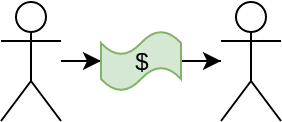
\includegraphics[width=0.7\textwidth]{b_ill1.png}
\end{figure}
\end{frame}

\begin{frame}[c]{Transaktion - Type 2}
\begin{figure}
	\centering
	\textbf{Distance Transaktion}\par\medskip
	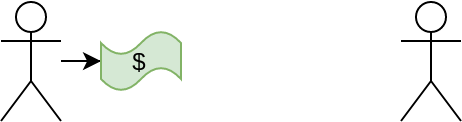
\includegraphics[width=0.7\textwidth]{b_ill2.png}
\end{figure}
\pause
\begin{block}{Problem}
	Hvordan overfører vi midler over distancer?
\end{block}
\end{frame}

\begin{frame}[c]{Transaktion - Mellemmand Løsning}
\begin{figure}
	\centering
	\textbf{Distance Transaktion}\par\medskip
	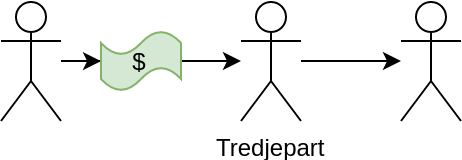
\includegraphics[width=0.7\textwidth]{b_ill3.png}
	\pause 
	\begin{block}{Tillidsløst Alternativ?}
		Finder der andre løsninger der ikke forudsætter tillid til tredjeparten?
	\end{block}
\end{figure}
\end{frame}

\begin{frame}[c]{blockchain?}
Blockchain teknologien har rejset utallige spørgsmål i medier de seneste år:
\begin{itemize}
	\item Hvordan virker den?
	\item Hvad kan teknologien bruges til?
	\item Sikker nok til at anvendes?
	\item Hvorfor skulle vi bruge den?
\end{itemize}
\end{frame}
\begin{frame}[c]{}
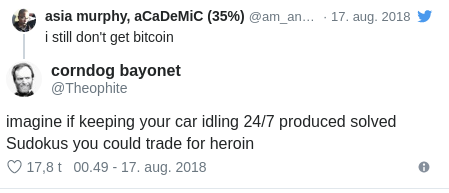
\includegraphics[width=1\textwidth]{bit.png}
\end{frame}


    \begin{frame}[c]{Ideen bag blockchain}
        \begin{quote}
            "A purely peer-to-peer version of electronic cash would allow online
            payments to be sent directly from one party to another without going through a
            financial institution." 
        \end{quote}
    	\rightline{{\rm --- Satoshi Nakamoto}}
    \end{frame}

    \begin{frame}[plain]{}
	    \begin{block}{Problem}
	    \textit{"Commerce on the Internet has come to rely almost exclusively on financial institutions serving as trusted third parties to process electronic payments."}\\
	    \end{block}
    	\pause
        \begin{enumerate}        	
        	\item Mægling omkostninger forøger transaktions omkostninger. 
        	\item Begrænset praktisk minimums grænse ved transaktioner, hvilket medfører færre små transaktioner.
        	\item Ingen ikke-reversible overførsler. 
        	\item Med reversible overførsler opstår behovet for tilled.
        \end{enumerate}
    \end{frame}

	\begin{frame}[plain]{}
		\begin{block}{Løsning}
			\textit{"What is needed is an electronic payment system based on cryptographic proof instead of trust, allowing any two willing parties to transact directly with each other without the need for a trusted	third party."} \\
		\end{block}
		\pause
		\begin{enumerate}        	
		\item Distribueret Netværk - globalt uden central styring, 
			\begin{itemize}
				\item Undgå mægling omkostninger
				\item ingen praktisk minimums grænse ved transaktioner
			\end{itemize}
		\item Kryptografisk bevis - stol på matematikken ikke personen.
			\begin{itemize}
				\item Tillidsfrit system
			\end{itemize}
		\item Blok struktur - Lænket og svært at forfalske.
			\begin{itemize}
				\item ikke-reversible overførsler - alt er hugget i sten
			\end{itemize}
		\end{enumerate}
	\end{frame}
	% ------------------------------------------------------------------------------

% ------------------------------------------------------------------------------
\section{De 3 hovedområder}
	\begin{frame}[plain]{Blockchain kerne områder}
	\hfill \break
	\hfill \break
	\begin{figure}
		\begin{minipage}[c]{0.1\textwidth}
			
\includegraphics[width=\textwidth]{disnet.png}
		\end{minipage}
		\begin{minipage}[c]{0.5\textwidth}
			\begin{itemize}
				\item Distribuerede database
			\end{itemize}
		\end{minipage}
	\end{figure}

		\begin{figure}
	\begin{minipage}[c]{0.1\textwidth}
		
\includegraphics[width=\textwidth]{blok.png}
	\end{minipage}
	\begin{minipage}[c]{0.5\textwidth}
		\begin{itemize}
			\item Blok struktur
		\end{itemize}
	\end{minipage}
\end{figure}
	
		\begin{figure}
		\begin{minipage}[c]{0.1\textwidth}
			
\includegraphics[width=\textwidth]{kon.png}
		\end{minipage}
		\begin{minipage}[c]{0.5\textwidth}
			\begin{itemize}
				\item Konsensus mekanisme
			\end{itemize}
		\end{minipage}
	\end{figure}
	\end{frame}

\begin{frame}{Database?}

\begin{block}{Hvad er en database?}
	\pause
	En måde at opbevare information på.
\end{block}
\begin{block}{Centraliserede vs Decentraliserede?}
	\pause
	\begin{itemize}
		\item \textbf{Central Database} - Al information holdes samlet og tilgås fra samme udgangspunkt.
		\item \textbf{Decentraliseret Database} - Information spredt ud over flere lokationer, forskellige arkitekturer. 
	\end{itemize}
\end{block}

\end{frame}
\begin{frame}{Centraliserede Database}
\begin{figure}
	\centering
	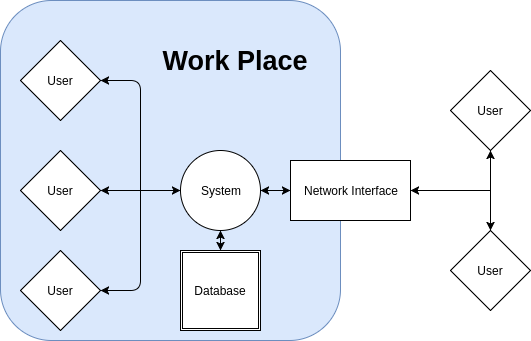
\includegraphics[width=0.9\textwidth]{CS.png}
	\caption{Centraliseret}
\end{figure}
\end{frame}

\begin{frame}{Decentraliserede Database}
\begin{figure}
	\centering
	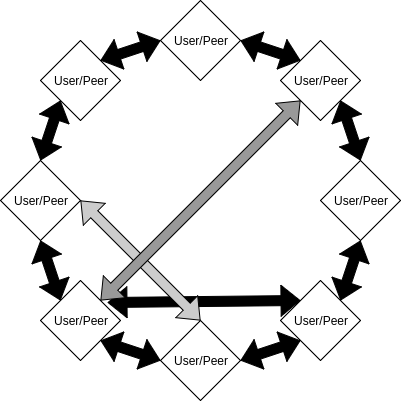
\includegraphics[width=0.7\textwidth]{dd.png}
	\caption{Decentraliseret}
\end{figure}
\end{frame}

\begin{frame}{Decentraliseret Vs Centraliseret}
\begin{figure}
	\centering
	\begin{subfigure}[b]{0.45\textwidth}
		\centering
		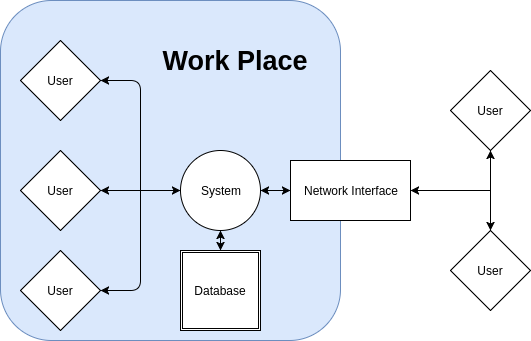
\includegraphics[width=1\textwidth]{CS.png}
		\caption{Centraliseret}
	\end{subfigure}
	\begin{subfigure}[b]{0.45\textwidth}
		
		\centering
	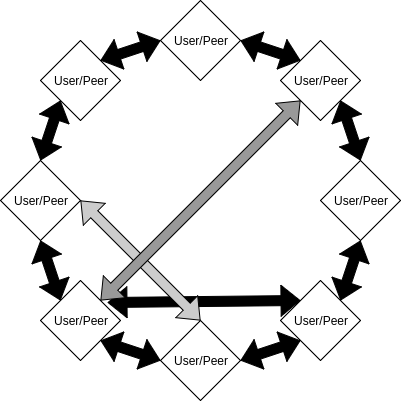
\includegraphics[width=0.7\textwidth]{dd.png}
	\caption{Decentraliseret}
	\end{subfigure}
\end{figure}
\begin{block}{Pros and Cons? }
	Hvilke fordele og ulemper er der ved brug af centrale kontra decentaliserede databaser? 
\end{block}
\end{frame}

\begin{frame}{Decentraliseret $\not =$ Distribueret}
\begin{figure}
	\centering
	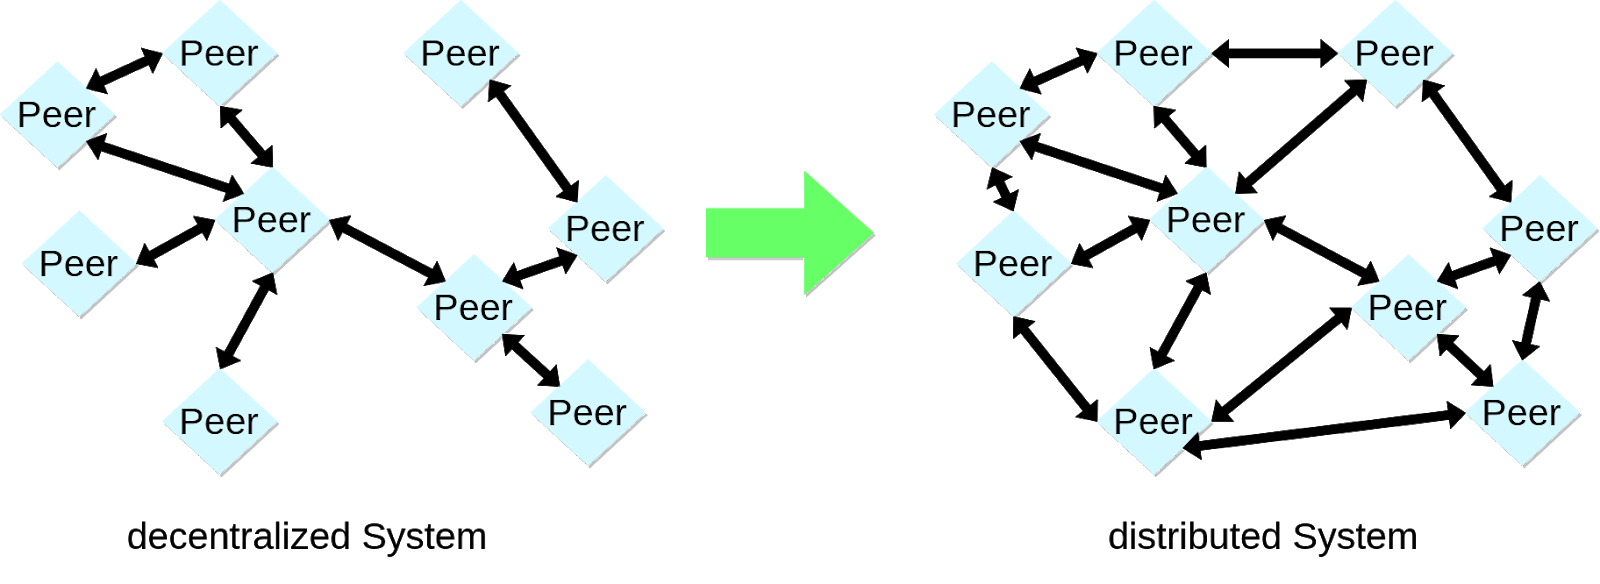
\includegraphics[width=1\textwidth]{centri.png}
\end{figure}
\begin{figure}
\begin{minipage}[c]{0.45\textwidth}
	\begin{itemize}
		\item Splittet Database
		\item Mist-bar Data
		\item Få updates
	\end{itemize}
\end{minipage}
\begin{minipage}[c]{0.45\textwidth}
	\begin{itemize}
		\item Spejlet Database
		\item Sikker Data
		\item Utallige updates
	\end{itemize}
\end{minipage}
\end{figure}
\end{frame}

\begin{frame}{Data Struktur}

\begin{block}{Hvad er en Data Struktur?}
	\pause
	En betegnelse for data det er struktureret i elementer, således at disse kan tilføjes eller fjernes.
\end{block}
\pause
Eksempler:
\begin{itemize}
	\item \textbf{Array} - Simpel datastruktur indelt efter en specifik orden.
	\item \textbf{Linked List} - Data struktur hvor hvert element, eller "node", henviser til det næste element i listen. 
	\item \textbf{Hash maps} - Data struktur formet efter navn og værdi, ingen specifik orden men yderst brugbart som opslagsværk.
\end{itemize}
\end{frame}

\begin{frame}{Linked list}
\begin{figure}
	\centering
	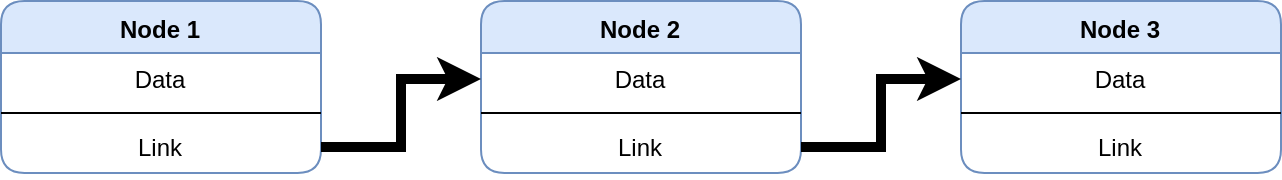
\includegraphics[width=1.1\textwidth]{ll.png}
	\caption{Linked List}
\end{figure}

\begin{block}{Brugbart i vores tilfælde?}
	Sammensætning af data på denne måde via referencer giver en  manøvrerbar strøm af data. Man kunne også kalde dette for en kæde? 
\end{block}
\end{frame}

\begin{frame}{Blok Data}
\begin{figure}
	\centering
	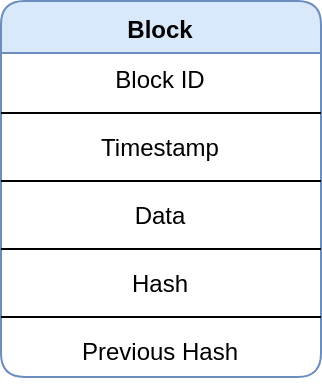
\includegraphics[width=0.5\textwidth]{block.png}
	\caption{Data Blok}
\end{figure}
\end{frame}

\begin{frame}{Blok Struktur}
\begin{figure}
	\centering
	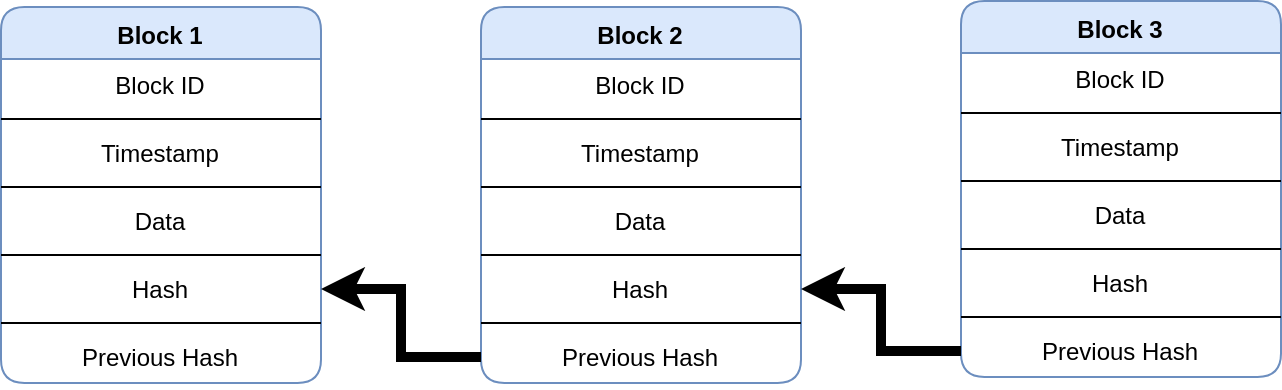
\includegraphics[width=1\textwidth]{bc.png}
	\caption{Bloks}
\end{figure}

\begin{block}{Sikker nok?}
	Selvom vi nu har defineret en brugbar struktur mangler vi stadig en måde hvorpå vi kan garantere data'en ikke bliver ændret.
\end{block}
\end{frame}

\begin{frame}{Konsensus Algoritme?}
\begin{block}{Hvad er en Algoritme?}
	En matematisk opskrift.	
\end{block}
\begin{block}{Konsensus?}
	En konsensus algoritme bruges til at garantere at datastrukturen forbliver u-kompromitteret 	
\end{block}
\begin{block}{Hashing?}
	Hashing er en måde hvorpå man omdanner data til en mindre billedmængde.\\ F.eks. ved brug af en sha-1 kan man omdanne:
	\begin{align*}
	\texttt{Hello World} \rightarrow \texttt{Sha-1} \rightarrow  \texttt{0a4d55a8d778e5022...}
	\end{align*}
\end{block}
\end{frame}


\begin{frame}
\begin{block}{Proof of Work - Algoritme}
	\vspace{-1.5em}
	\begin{algorithm}[H]
		\caption{\newline Input: Problem, data
			\newline Output: Hash
		}
		\begin{algorithmic}
			\State hash = Hash\_Funktion(data)
			\State nonce = 0
			\While{Hash $\not =$ Problem}
			\State nonce += 1
			\State data += nonce
			\EndWhile
			\State 	Return hash
		\end{algorithmic}
	\end{algorithm}
\end{block}
\end{frame}

\begin{frame}{Proof of Work}
\begin{figure}
	\centering
	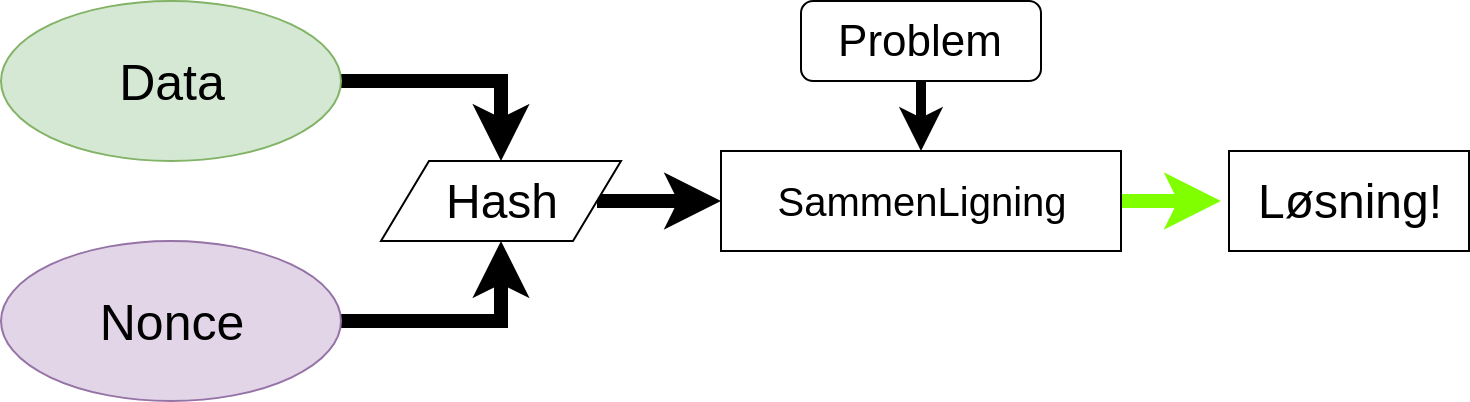
\includegraphics[width=1.1\textwidth]{pow.png}
\end{figure}
\end{frame}
\begin{frame}{Proof of Work}
\begin{figure}
	\centering
	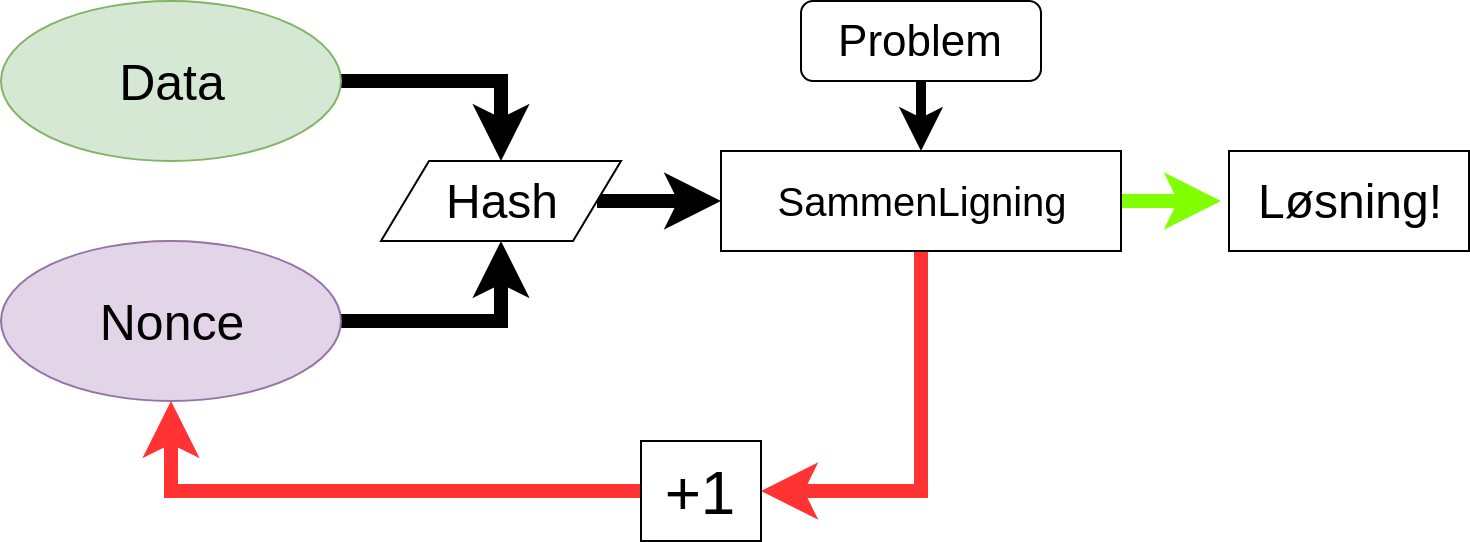
\includegraphics[width=1.1\textwidth]{pow2.png}
\end{figure}
\end{frame}

\begin{frame}{Konsensus Algoritme/mekanismer - Alternativer}
\begin{block}{Der findes et antal alternativer til "Proof of Work"}
	\begin{itemize}
		\item Proof of Stake (PoS)
		\begin{itemize}
			\item Belægger sig på brugerens værdi, jo større værdi jo større chance for at tilføje den næste blok.
		\end{itemize}
		\item Proof of Elapsed Time (PoET)
		\begin{itemize}
			\item Bruges i \textit{"Permissional Blockchains"}, fungere ved at hver "node" venter på det bliver deres tur til at "commit" en block til kæden. 
		\end{itemize}
		\item Proof of Authority (PoA)
		\begin{itemize}
			\item Bruges i mindre blockchain systemer, her vælges et antal brugere som "validators", og giver dem alene magten til at autorisere nye blokke.
		\end{itemize}
	\end{itemize}
\end{block}
\end{frame}

% ------------------------------------------------------------------------------

% ------------------------------------------------------------------------------

\section{Anvendelses Muligheder}

\begin{frame}{Kun Krypto Valuta?}
	\begin{figure}
	\centering
	\begin{subfigure}[b]{0.45\textwidth}
		\centering
		
\includegraphics[width=1\textwidth]{tracr.png}
		\caption{Tracr - Diamond Track}
	\end{subfigure}
	\begin{subfigure}[b]{0.45\textwidth}
		
		\centering
		
\includegraphics[width=0.65\textwidth]{uport.png}
		\caption{Uport - Zug ID}
	\end{subfigure}
\end{figure}
\end{frame}

\section{Opsamling og Spørgsmål}
    \begin{frame}[c]{Spørgsmål}
        \begin{quote}
            \centering Nogen spørgsmål?
        \end{quote}
    \end{frame}
% ------------------------------------------------------------------------------

\end{document}
